\documentclass[12pt]{beamer}

%\documentclass[a4paper,12pt,spanish,oneside]{book}
\usepackage{amsmath}
\usepackage{amsthm}
\usepackage{amssymb}
\usepackage{enumerate}
\usepackage{verbatim}
\usepackage{makeidx}
% \usepackage{stmaryrd}

\usepackage[utf8]{inputenc}
\usepackage[spanish]{babel}
%\usepackage[latin1]{inputenc}
%\usepackage{t1enc}

\newlength{\ancho}
\setlength{\ancho}{\paperwidth}
\addtolength{\ancho}{-2in}
\textwidth=\ancho
%\topmargin=0pt
%\headsep=0pt
%\headheight=0pt
%\evensidemargin=0mm
%\oddsidemargin=0mm

%
%Caracteres

\newcommand{\Baire}{\mathcal N}
\newcommand{\Cantor}{\mathcal C}
\newcommand{\R}{\mathbb R}
\newcommand{\C}{\mathbb C}
\newcommand{\Q}{\mathbb Q}
\newcommand{\N}{\mathbb N}
\newcommand{\I}{\mathbb I}
\newcommand{\Qvar}{\mathcal Q}
\newcommand{\K}{\mathcal K}
\newcommand{\T}{\mathcal T}
\newcommand{\U}{\mathcal U}
\newcommand{\F}{\mathcal F}

%Varias
\newcommand{\subp}{\mathrm{M}}
\newcommand{\prob}{\mathrm{P}}
\newcommand{\graf}{\mathrm{graf}}
\newcommand{\diam}{\mathrm{diam}}
\newcommand{\B}{\mathbf{B}}
\newcommand{\longi}{\mathrm{long}}
\newcommand{\osc}{\mathrm{osc}}
\newcommand{\tends}{\rightarrow}

%
%	Estilo
\newcommand{\mc}[1]{\mathcal{#1}}
\newcommand{\mb}[1]{\mathbf{#1}}
\newcommand{\remark}[1]{\marginpar{\tiny{#1}}}
\renewcommand{\eqref}[1]{(\ref{#1})}
\newcommand{\teoref}[1]{teorema \ref{#1}}
\newcommand{\propref}[1]{proposicin \ref{#1}}
\newcommand{\lemaref}[1]{lema \ref{#1}}
\newcommand{\cororef}[1]{corolario \ref{#1}}

%
% 	Logicas
\newcommand{\true}{\mathsf{T}}
\newcommand{\sat}{\vDash}
\newcommand{\nsat}{\nvDash}
\newcommand{\sii}{\Leftrightarrow}
\newcommand{\logeq}{\Leftrightarrow}
\newcommand{\ent}{\rightarrow}
\newcommand{\tne}{\Leftarrow}
\newcommand{\iso}{\cong}		
\newcommand{\func}{\rightarrow}
\newcommand{\Func}{\longrightarrow}
\newcommand{\comp}{\circ}
\newcommand{\y}{\wedge}
\newcommand{\Y}{\bigwedge}
\renewcommand{\o}{\vee}
\newcommand{\abst}[1]{\llbracket #1\rrbracket}

% USO: \equ{i}{x} ---> p_i(x) = q_i(x)
\newcommand{\equ}[2]{p_{#1}(\vec{#2})=q_{#1}(\vec{#2})}

% USO: \quasiid{i}{x}
%\newcommand{\quasiid}[2]{\forall \vec{#2}(\Y_{#1=1}^n \equ{#1}{#2}) \ent \equ{}{#2}}
\newcommand{\quasiid}[2]{\forall \vec{#2}([(\Y_{#1=1}^n p_#1 = q_#1) \ent p = q]\vec{#2}}

% USO: \quasiid{n}
%\newcommand{\qi}[1]{\mathrm{qid}(p_1,q_1,\ldots,p_#1,q_#1,p,q)}
\newcommand{\qi}[1]{\mathrm{qid}(\{(p_i,q_i)\}_{i=1}^#1,p,q)}

%quasivariedad generada
\newcommand{\qgen}[1]{\mathrm{Q}(#1)}

%congruencia identidad
\newcommand{\id}[1]{\Delta^#1}

%
% Conjuntos
\newcommand{\union}{\ensuremath{\cup}}
\newcommand{\Union}{\ensuremath{\bigcup}}
\newcommand{\included}{\ensuremath{\subseteq}}
\newcommand{\includes}{\ensuremath{\supseteq}}
\newcommand{\notincluded}{\ensuremath{\not\subseteq}}
\newcommand{\inters}{\ensuremath{\cap}}
\newcommand{\Inters}{\ensuremath{\bigcap}}
\newcommand{\en}{\ensuremath{\in}}
\newcommand{\foral}{\ensuremath{\forall}}
\newcommand{\exi}{\ensuremath{\exists}}
\newcommand{\subi}[1]{\ensuremath{_{#1}}}
\newcommand{\compl}[1]{#1^c}
\newcommand{\f}[3]{{#1:#2\rightarrow#3}}
\newcommand{\vacio}{\emptyset}
\newcommand{\dom}{\mathrm{dom}}
\newcommand{\Pfin}{P^{<\omega}}

%
%	Griegas
\renewcommand{\th}{\theta}
\renewcommand{\a}{\alpha}
\renewcommand{\b}{\beta}
\newcommand{\g}{\gamma}
\newcommand{\Ga}{\Gamma}
\renewcommand{\d}{\delta}
\newcommand{\eps}{\epsilon}
\newcommand{\e}{\varepsilon}
\newcommand{\vp}{\varphi}
\newcommand{\sig}{\sigma}
\newcommand{\Sig}{\Sigma}
\renewcommand{\l}{\lambda}
\newcommand{\La}{\Lambda}
\newcommand{\om}{\omega}
\newcommand{\Om}{\Omega}
\newcommand{\z}{\zeta}

%
%	Entornos de redaccion
\newenvironment{dem}{\begin{proof}[Prueba]}{\end{proof}}
\newenvironment{ideadem}{\begin{proof}[Idea de prueba]}{\end{proof}}
\newenvironment{sol}{\begin{proof}[Solución]}{\end{proof}}
%
\theoremstyle{definition}
\newtheorem{defn}{Definición}
%
\theoremstyle{remark}
\newtheorem{ejem}{Ejemplo}
\newtheorem{nota}{Nota}
\newtheorem{observ}{Observación}
%
\theoremstyle{plain}
\newtheorem{lem}{Lema}
\newtheorem{af}[lem]{Afirmación}
\newtheorem{teo}[lem]{Teorema}
\newtheorem{coro}[lem]{Corolario}
\newtheorem{prop}[lem]{Proposición}


%%%%%%%%%%% Lo que viene  a continuacion es el tipo de presentacion que quieres, 
% las presentaciones se llaman con nombres de ciudades puedes cambiarlas y tomar
%%%%%%%%la que mas te guste.
\mode<presentation> {
  %\usetheme{Frankfurt}
  %\usetheme{Warsaw}
  %\usetheme{Darmstadt}
   \usetheme{Dresden}
%   \usetheme{Singapore}
  %\usetheme{Bergen}
  %\usetheme{Boadilla}
  %\usetheme{BerKeley}
  \setbeamercovered{transparent}
  %\setbeamertemplate{background canvas}[vertical shading][bottom=red!20,top=yellow!30]
%   \setbeamertemplate{headline}{}
%%%%%%%%%%%%%%%%%%%%%%%%%%%%%%%%%%
%%%%%%% aqui vienen los colores

  %\usecolortheme{crane}
  %\usecolortheme{seahorse}
  \usecolortheme{whale}
  %\usecolortheme{rose}
  %\usecolortheme{orchid}
} \usepackage{alltt}

\newenvironment{stepenumerate}{\begin{enumerate}[<+->]}{\end{enumerate}}
\newenvironment{stepitemize}{\begin{itemize}[<+->]}{\end{itemize} }
\newenvironment{stepenumeratewithalert}{\begin{enumerate}[<+-| alert@+>]}{\end{enumerate}}
\newenvironment{stepitemizewithalert}{\begin{itemize}[<+-| alert@+>]}{\end{itemize} }
\newtheorem{propo}{Proposition}

%%%%%%%los paquetes. 
\usepackage{amssymb,amsmath,latexsym}
%\usepackage[mathcal]{euscript}
%\usepackage[polish]{babel}
\usepackage{color}
\usepackage{hyperref}
%\usepackage{dsfont}
%\usepackage[normalem]{ulem}
\usepackage{enumerate}
%\usepackage[all,2cell,dvips]{xy} \UseAllTwocells \SilentMatrices
\usepackage[utf8]{inputenc}
\usepackage[spanish]{babel}
\usepackage{verbatim}
\usepackage{float}

\title{Análisis de la herramienta TLA+ Proof System}
%
%
\author{Pablo Celayes, Giovanni Rescia, Ariel Wolfmann}

%
\institute{Facultad de Matemática, Astronomía y Física\\
Universidad Nacional de Córdoba}

\date{Junio 2015}


\begin{document}
%%%%%%%%%%%%%%%%%%%%%%%%%%%PAGINA DEL TITULO
\begin{frame}
  \titlepage
\end{frame}

%%%%%%%%%%%%%%%%%  tODO LO QUE QUIERAS PONER EN LOS FRAMES.
\begin{frame}
  \frametitle{Veremos...}
  \tableofcontents[pausesections]
\end{frame}
  %  \tableofcontents[pausesections]
%   %You might wish to add the option [pausesections]


%%%%%%%%%%%%%%%%%%%%%%%% EFDs & Algebraic Functions %%%%%%%%%%%%%%%%%%%%%%%%%%%%
\section{Contexto}
\begin{frame}{1977}
  Pnueli introduce su lógica temporal para describir sistemas.
  \pause
  \begin{stepitemize}
    \item útil para ciertas propiedades, limitada para otras
    \item se combinaba con formas más tradicionales de descripción
  \end{stepitemize}
\end{frame}	
	
\begin{frame}{fin de los 80's}
  Lamport introduce TLA
  \pause
  \begin{stepitemize}
    \item variante de la lógica temporal de Pnueli
    \item mayormente notación matemática tradicional
    \item lógica temporal sólo donde es imprescindible  
  \end{stepitemize}
\end{frame}	

\begin{frame}{2001...}
  Lamport se va a Microsoft Research
  \pause
  \begin{stepitemize}
    \item Surge TLA+ (extensión de TLA para escribir \textbf{pruebas})
    \item Desarrollo del \textbf{Toolbox} y el {TLA+ Proof System}
  \end{stepitemize}
\end{frame}
	
\begin{frame}{...2015}
  \textit{Tools for Proofs}
  \pause
  \begin{stepitemize}
    \item Colaboración Microsoft - INRIA
    \item Proyecto activo (issue tracker, mailing list)
    \item Aplicación en academia e industria
  \end{stepitemize}
\end{frame}

\section{Objetivos}
\begin{frame}
\begin{stepitemize}
 \item TLAPS permite verificar la correctitud de pruebas escritas en TLA+
 \item Una prueba en TLA+ es una colección de sentencias con jerarquía. TLAPS comprueba que dicha jerarquía implican de hecho la correctitud del teorema a demostrar
\end{stepitemize}
\end{frame}


\section[Descripción]{Descripción del lado del usuario}
\begin{frame}
    Posee un IDE \textbf{Toolbox}, que integra las siguientes herramientas:
      \begin{stepitemize}
	\item \textbf{PlusCal}: Lenguaje algoritmico simple que se compila a TLA+
	\item \textbf{Modelo Standard}: Un sistema se describe como un conjunto de comportamientos
	\item \textbf{TLC}: \textit{Model Checker}
	\item \textbf{TLA+ Proof System}: Desarrollo y verificación mecánica de demostraciones
      \end{stepitemize}

\end{frame}


\section{Aspectos técnicos}
\begin{frame}
\frametitle{Aspectos técnicos}
  Una especificación en TLA+ es un módulo raíz, que puede importar otros módulos por extensión e instanciación de sus respectivos parámetros.
  \pause
  
  La arquitectura de TLAPS se divide en:
  \begin{itemize}
    \item TLAPM
    \item Backends
  \end{itemize}

\end{frame}

\begin{frame}
 \frametitle{TLAPM}
  Se encarga de:
 \begin{stepitemize}
  \item Expandir e instanciar módulos (usando estado implícito)
  \item Generar obligaciones de prueba
  \item Invocar a los backends para verificar las obligaciones de pruebas
  \item Generar estructura del lema
  \item Generar prueba del teorema usando las obligaciones ya certificadas
 \end{stepitemize}
\end{frame}

\begin{frame}
 \frametitle{Backends}
 Para corroborar una obligación de prueba, el comportamiento por defecto de TLAPS es probar con 3 backends en sucesión: 
 \pause
 \begin{stepitemize}
  \item SMT: invocado por defecto, timeout: 5 segundos
  \item Zenon: lógica de primer orden, timeout: 10 segundos
  \item Isa: probador automático de Isabelle, timeout: 30 segundos
 \end{stepitemize}
 \pause
  Si Isabelle no puede encontrar una prueba, TLAPS (por medio de TLAPM) reporta una falla al intentar demostrar dicha obligación.
\end{frame}

\begin{frame}
  \begin{figure}
    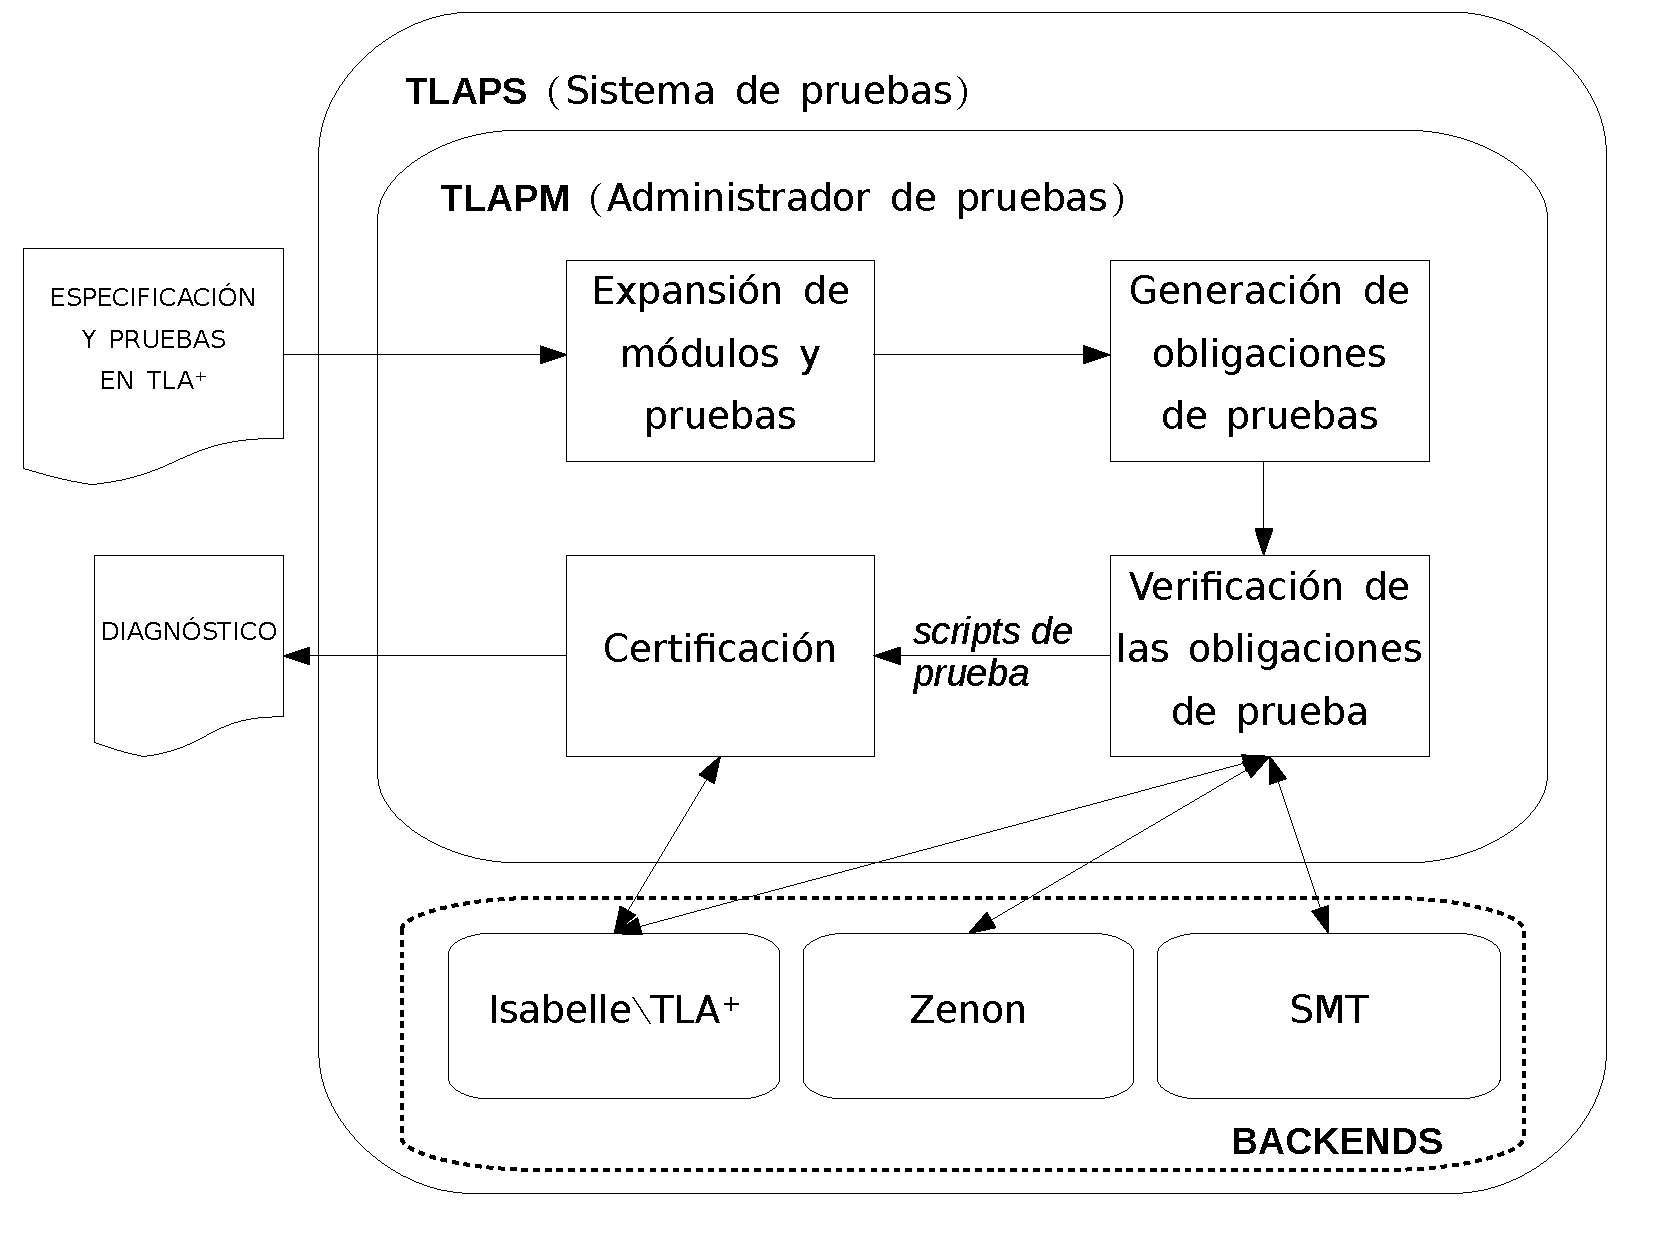
\includegraphics[scale=0.30]{esquema-informe-ingsoft2}
    
    Arquitectura general de TLAPS
  \end{figure}
 \end{frame}


\section[Casos]{Casos de aplicación}
\begin{frame}
  \begin{stepitemize}
    \item Amazon
      \begin{itemize}
      \item DynamoDB, S3, EBS
      \item Bugs críticos pero sutiles: ¡trazas de hasta \textbf{35} pasos!
      \item creciente adopción en la empresa
      \end{itemize}
    \item XBOX 360 
      \begin{itemize}
       \item bug \textbf{crítico} en sistema de memoria
       \item lo descubrió un pasante con TLA+
       \item cada \texit{XBOX 360} se habría colgado tras 4 horas de uso
      \end{itemize}
  \end{stepitemize}
\end{frame}

\begin{frame}
  \begin{stepitemize}
    \item Farsite
      \begin{itemize}
	\item Sistema de archivos distribuido $\approx$ NTFS
	\item TLA+ para especificar y verificar propiedades concurrentes
      \end{itemize}
    \item Byzantine Paxos
      \begin{itemize}
      \item Tolerancia a fallas maliciosas en sistemas distribuidos
      \item Prueba formal
      \end{itemize}
  \end{stepitemize}
\end{frame}


\section[Comparaciones]{Comparación con otras herramientas}
\begin{frame}
\frametitle{TLA+ vs Alloy}
    \begin{stepitemize}
      \item Concepto de modelado similar
      \item TLA+ es mucho mas expresivo que Alloy
      \item Importancia en la práctica
      \item Muchas especificaciones reales escritas en TLA+ son casi imposibles de escribir en Alloy
    \end{stepitemize}

\end{frame}

\begin{frame}

  \frametitle{herramientas similares a TLAPS}
  \begin{stepitemize}
	  \item Isar
	  \begin{itemize}
	    \item Corre sobre Isabelle
	    \item Estilo de desarrollo diferente
	    \item Bueno para pruebas cortas pero no tanto para pruebas largas
	   \end{itemize}
	   \item Focal
	    \begin{itemize}
	     \item Subconjunto de TLA+, que incluye el desarrollo de demostraciones jerárquicamente. 
	    \end{itemize}
	   \item Coq
	   \begin{itemize}
	    \item Corre sobre Zenon
	    \item Desarrollo semi-interactivo
	   \end{itemize}

	    

  \end{stepitemize}


\end{frame}

\section{Ejemplo}
\begin{frame}
correctitud del algoritmo de Euclides
\end{frame}

\section{Conclusiones}
\begin{frame}{Conclusiones}
%%%%%%%
  \begin{stepitemize}
  \item TLA+ : 
  	   \begin{itemize}
	    \item Simple pero expresivo (notación matemática simple)
	    \item Toolbox facilita interacción
	    \item Buena aceptación en la industria
	   \end{itemize}
  \item TLAPS: 
    	   \begin{itemize}
	    \item Ventaja de TLA+ sobre otros \textit{Model Checkers}
	    \item Demasiado específico $\rightarrow$ Poco uso en la industria
	   \end{itemize}
  \end{stepitemize}
\end{frame}

\begin{frame}
 {\Huge ¿Preguntas?}
\end{frame}

\begin{frame}
 {\Huge ¡Gracias por escuchar!}
\end{frame}



% \begin{frame}%%%%%%%%%%
% \frametitle{Referencias}
% \begin{thebibliography}
% 
% %\pause
% \bibitem[KrCla79]{AE-classes}\textrm{Krauss, P.H., Clark, D.M.}, 
% \textit{Global Subdirect Products}, Amer. Math. Soc. Mem. \textbf{210} (1979).
% 
% 
% \end{thebibliography}
% 
% \end{frame}

\begin{frame}
\begin{figure}[center]
% \includegraphics[width=95mm]{19127354.jpg}
%\caption{algebraically closed clones in Post's Lattice} 
\end{figure}
\end{frame}

\end{document}
